\chapter{HARDWARE IMPLEMENTATION AND MECHANICAL FABRICATION}
\label{ch:hardware_mechanical}

\section{Microcontroller Unit: 7Semi ESP32-DEVKIT-E Architecture}
The processing core of VibeGuard is the \textbf{7Semi ESP32-DEVKIT-E} development board, carrying an integrated Espressif ESP32-WROOM-32E system-in-package module. Selected for its computational power, deterministic peripheral timing, and low power consumption, the microcontroller provides the necessary hardware foundation for real-time edge vibration analytics~\cite{esp32_devkitc_guide}.

\begin{table}[H]
\centering
\begin{tabular}{|l|l|}
\hline
\textbf{Hardware Feature} & \textbf{Architectural Specification} \\
\hline
Processor Core & 32-bit Dual-Core Xtensa LX6 Microprocessor \\
Clock Frequency & Up to 240\,MHz (Configured at 160\,MHz for thermal stability) \\
Internal SRAM & 520\,KB on-chip SRAM (Sufficient for FFT scratch buffers) \\
External Flash Memory & 4\,MB SPI Flash (For firmware storage and frozen calibration tables) \\
USB-to-UART Bridge & Silicon Labs CP2102 (Supports baud rates up to 921,600\,baud) \\
Voltage Regulator & AMS1117-3.3 (800\,mA maximum output, thermal overload protection) \\
Hardware Timers & Four 64-bit general-purpose hardware timers \\
Dedicated SPI Controllers & 2 available (VSPI utilized for ADXL345 sensor bus) \\
Operating Supply Voltage & 5.0\,V via Micro-USB (Regulated to 3.3\,V on-carrier) \\
\hline
\end{tabular}
\caption{7Semi ESP32-DEVKIT-E architectural specifications}
\label{tab:esp32_specs}
\end{table}

\subsection{Physical Form Factor and Breadboard Clearance}
The 7Semi board employs the industry-standard 38-pin DevKitC V4 dual-inline physical header layout. The pin row spacing measures exactly 22.86\,mm (0.90\,inches). When inserted across the center divider trench of a standard MB102 830-point solderless breadboard, the module leaves one full row of tie-points exposed along both lateral sides. This provides direct, reliable breadboard access for sensor bus jumper wires and diagnostic test probes without requiring awkward under-board bridging.

\section{Triaxial Digital Accelerometer: ADXL345}
The primary vibration transducer is the Analog Devices ADXL345, a micro-machined capacitive triaxial digital accelerometer~\cite{adxl345_datasheet}. 

\subsection{Internal Sensing Architecture}
The ADXL345 sensing element is fabricated from surface-micromachined polysilicon forming a differential capacitive beam structure. When subjected to acceleration along its sensitive axes, internal proof masses displace relative to stationary capacitor plates, altering differential capacitance. On-chip switched-capacitor synchronous demodulators convert capacitance shifts into proportional analog voltages. An integrated 13-bit sigma-delta ($\Sigma\Delta$) ADC converts the analog signals into two's-complement digital words.

\subsection{Operating Mode and Full-Resolution Scaling}
The ADXL345 is configured via firmware into \textbf{Full-Resolution Mode} with a $\pm 4g$ dynamic range setting. In this mode, the internal ADC resolution scales automatically with the dynamic range (11 bits at $\pm 4g$), maintaining a strictly constant sensitivity scale factor:
\begin{equation}
S = 3.9\,\text{mg / LSB} = 0.0039\,g/\text{LSB} = 0.03825\,\text{m/s}^2/\text{LSB}
\label{eq:scale_factor}
\end{equation}
Maintaining a constant $3.9\,\text{mg/LSB}$ scale factor eliminates dynamic range scaling artifacts and preserves arithmetic consistency across both baseline low-vibration and extreme unbalance operating regimes. 

The sensor's internal 32-level First-In First-Out (FIFO) buffer is configured in \textbf{Stream Mode}. In Stream Mode, the FIFO continuously buffers acceleration samples, automatically discarding the oldest data when full. This buffers transient interrupts and guarantees that the microcontroller never reads corrupted or partially updated register pairs.

\section{Drive Subsystem: 12V N20 Micro Metal Gear Motor}
Controlled vibration generation is provided by an industrial-grade \textbf{N20 Micro Metal Gear Motor}.
\begin{itemize}
    \item \textbf{Gearbox Architecture:} Incorporates an all-metal multi-stage spur gearbox with a 1:50 gear reduction ratio, delivering high torsional stiffness and eliminating gear backlash during continuous rotation.
    \item \textbf{Rotational Velocity:} At its rated 12.0\,V DC supply voltage, the motor rotates at a stable 600\,RPM, establishing a clean $10.0$\,Hz fundamental mechanical excitation frequency.
    \item \textbf{D-Shaft Geometry:} The hardened steel output shaft features a precision D-shaft cross-section with an outer diameter of $3.00\,\text{mm} \pm 0.02\,\text{mm}$, a flat-to-back chord depth of $2.50\,\text{mm}$, and an axial length of $9.50\,\text{mm}$. The flat chord provides positive mechanical keying against rotor slippage.
\end{itemize}

\section{Mechanical Testbed Baseplate Design and Dual-Datum Drilling}
In vibration analysis, the structural rigidity and acoustic impedance of the mounting foundation are paramount. Flexible foundations flex dynamically under motor load, introducing spurious structural resonance modes that contaminate sensor readings.

\subsection{Laminated Acrylic Baseplate}
The VibeGuard testbed utilizes a 10.0\,mm thick laminated optical-grade cast polymethyl methacrylate (acrylic) baseplate measuring $150\,\text{mm} \times 150\,\text{mm}$. The total mass of the plate is approximately $265\,\text{g}$. Acrylic provides high mechanical damping, excellent dimensional stability, and superior stiffness compared to thin wood or hollow 3D-printed chassis.

\subsection{Dual-Datum Drilling Matrix}
To guarantee repeatable alignment between the motor output shaft, eccentric rotor, and accelerometer mount, the baseplate features eight precision 3.0\,mm through-holes drilled according to a certified dual-datum coordinate system. Figure~\ref{fig:baseplate_blueprint} illustrates the master mechanical drilling blueprint.

\begin{figure}[H]
\centering
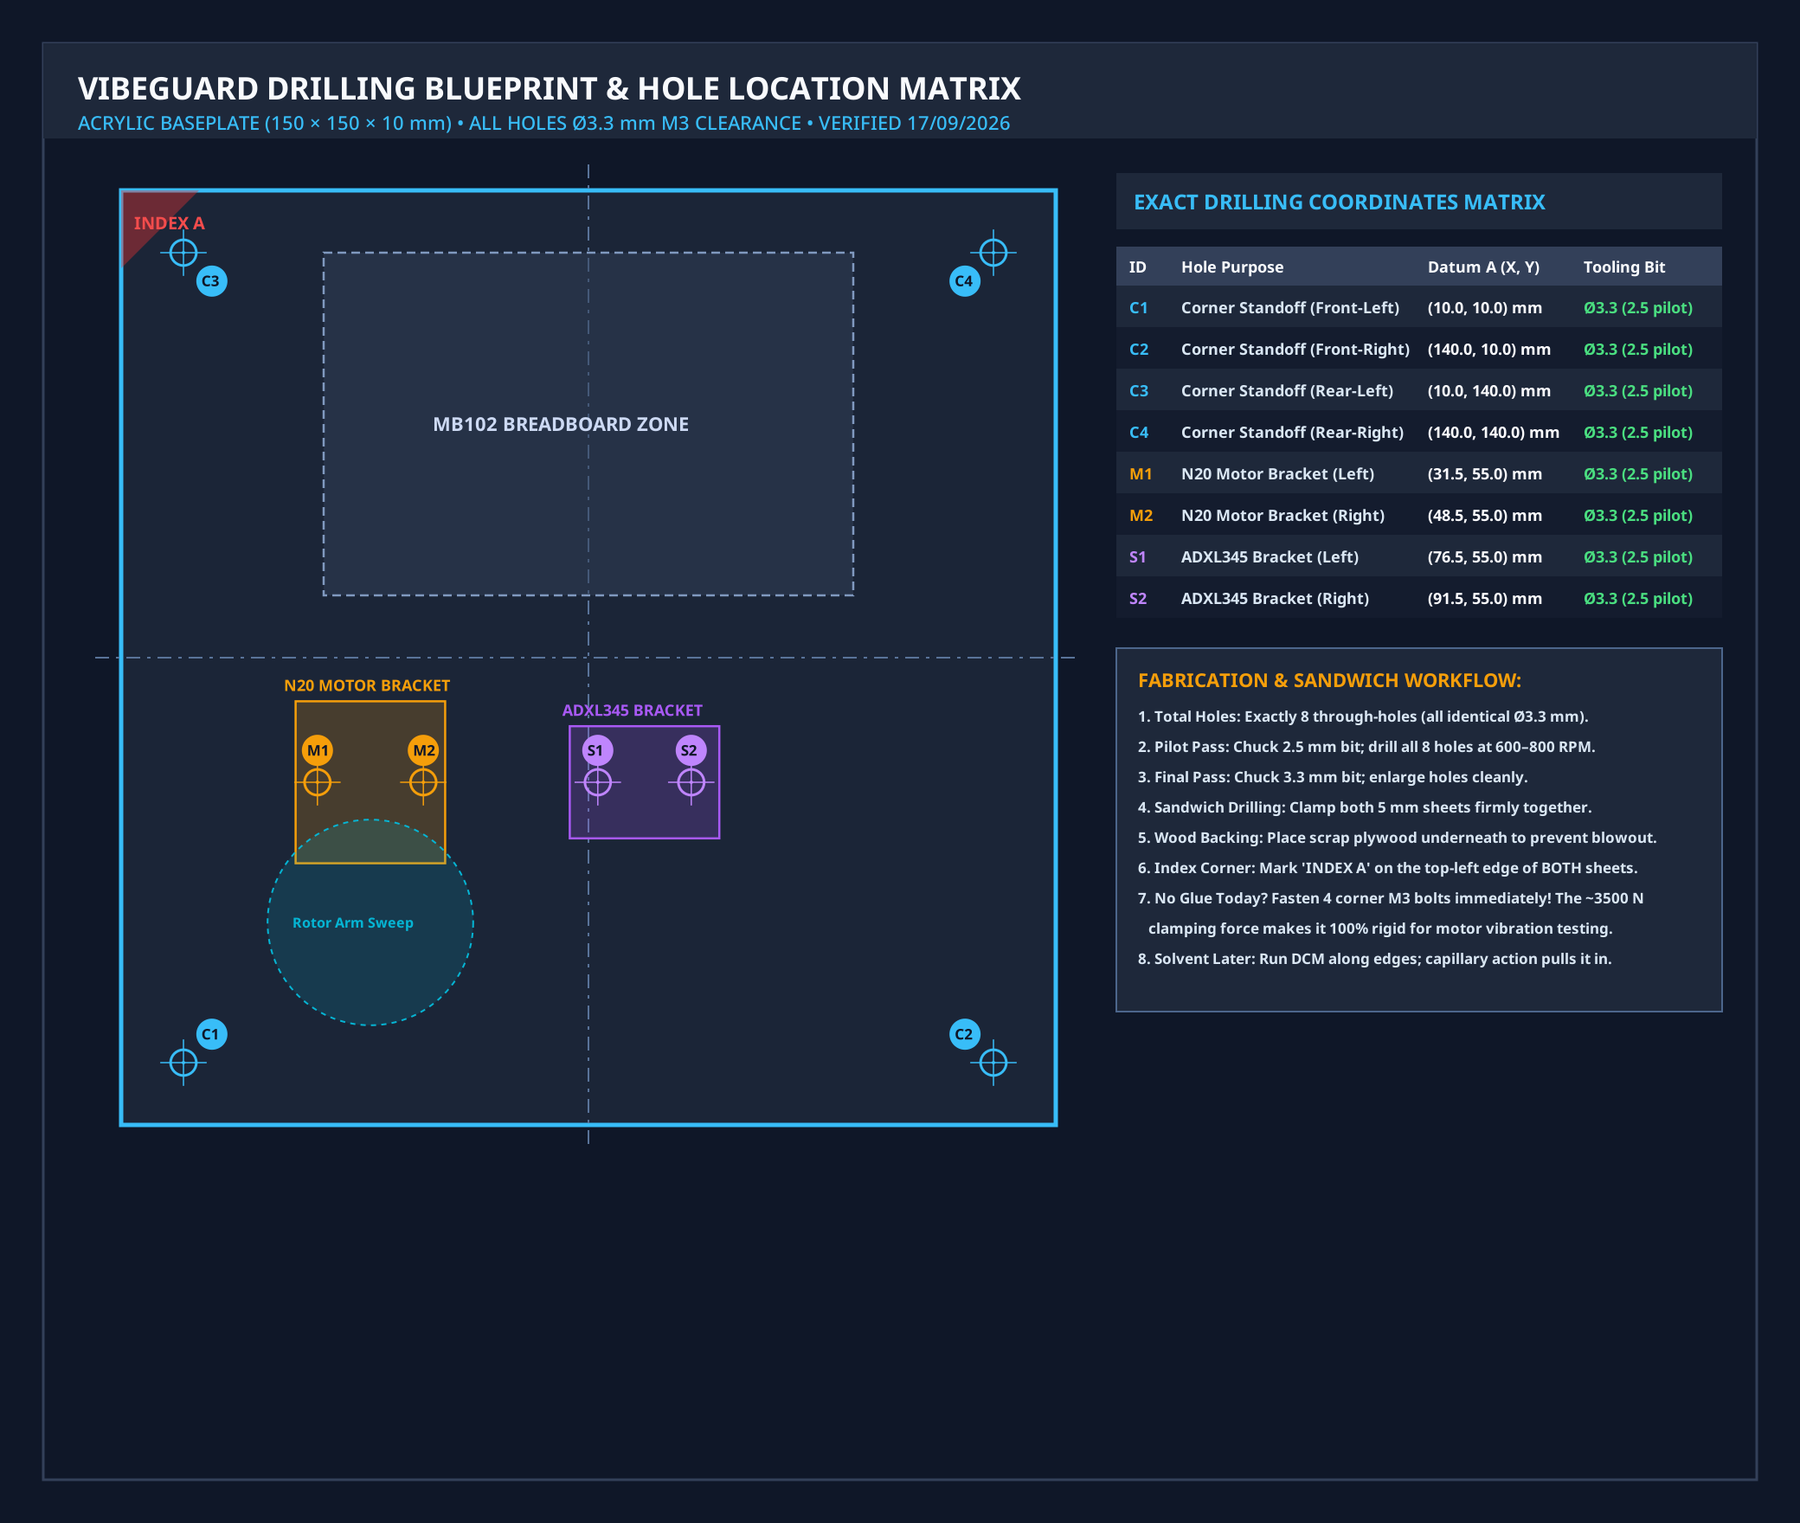
\includegraphics[width=0.88\textwidth]{figures/fig_baseplate_blueprint.png}
\caption{Certified 1:1 mechanical baseplate fabrication blueprint with dual-datum dimensions}
\label{fig:baseplate_blueprint}
\end{figure}

The hole layout incorporates two complementary reference coordinate systems:
\begin{enumerate}
    \item \textbf{Center-Referenced Coordinates $(X_c, Y_c)$:} Origin $(0,0)$ located at the geometric center of the $150 \times 150$\,mm plate.
    \item \textbf{Corner Datum Coordinates $(X_d, Y_d)$:} Origin $(0,0)$ located at the bottom-left corner of the acrylic sheet, facilitating physical manual marking using workshop vernier calipers.
\end{enumerate}

Table~\ref{tab:drilling_matrix} lists the complete dimensional matrix for all eight mounting holes.

\begin{table}[H]
\centering
\small
\begin{tabular}{|l|c|c|c|c|c|}
\hline
\textbf{Mounting Feature} & \textbf{$X_c$ (mm)} & \textbf{$Y_c$ (mm)} & \textbf{$X_d$ (mm)} & \textbf{$Y_d$ (mm)} & \textbf{Fastener} \\
\hline
Corner Foot 1 (Bottom-Left) & $-65.0$ & $-65.0$ & $+10.0$ & $+10.0$ & M3 Bolt / Rubber Pad \\
Corner Foot 2 (Bottom-Right) & $+65.0$ & $-65.0$ & $+140.0$ & $+10.0$ & M3 Bolt / Rubber Pad \\
Corner Foot 3 (Top-Left) & $-65.0$ & $+65.0$ & $+10.0$ & $+140.0$ & M3 Bolt / Rubber Pad \\
Corner Foot 4 (Top-Right) & $+65.0$ & $+65.0$ & $+140.0$ & $+140.0$ & M3 Bolt / Rubber Pad \\
\hline
N20 Motor Bracket Hole 1 & $+14.0$ & $-5.5$ & $+89.0$ & $+69.5$ & M3 $\times$ 20\,mm Through-Bolt \\
N20 Motor Bracket Hole 2 & $+14.0$ & $+5.5$ & $+89.0$ & $+80.5$ & M3 $\times$ 20\,mm Through-Bolt \\
ADXL345 Sensor Stand Hole 1 & $-20.0$ & $-7.5$ & $+55.0$ & $+67.5$ & M3 $\times$ 20\,mm Through-Bolt \\
ADXL345 Sensor Stand Hole 2 & $-20.0$ & $+7.5$ & $+55.0$ & $+82.5$ & M3 $\times$ 20\,mm Through-Bolt \\
\hline
\end{tabular}
\caption{Certified baseplate dual-datum drilling coordinate matrix}
\label{tab:drilling_matrix}
\end{table}

Key geometric relationships certified by this layout include:
\begin{itemize}
    \item \textbf{Motor Hole Pitch:} Exactly 11.0\,mm center-to-center spacing along the $Y$-axis.
    \item \textbf{Sensor Hole Pitch:} Exactly 15.0\,mm center-to-center spacing along the $Y$-axis.
    \item \textbf{Parallel Clearance Gap:} A 34.0\,mm centerline separation along the $X$-axis between the motor bracket line ($X = +14.0$\,mm) and sensor mount line ($X = -20.0$\,mm), ensuring a clean 20.0\,mm physical air gap between the spinning rotor arm and the sensor upright.
\end{itemize}

\section{3D-Printed Monolithic Rotor Cam Arm (FAB-01)}
In initial pilot testing, multi-part assembled rotor linkages separated physically under high-speed rotation due to centrifugal shear forces. To achieve absolute structural integrity, the eccentric rotor arm (\textbf{FAB-01}) was redesigned as a 100\% monolithic, single-piece solid model.

Figure~\ref{fig:rotor_arm} shows the 3D-rendered solid model of the FAB-01 rotor cam arm.

\begin{figure}[H]
\centering
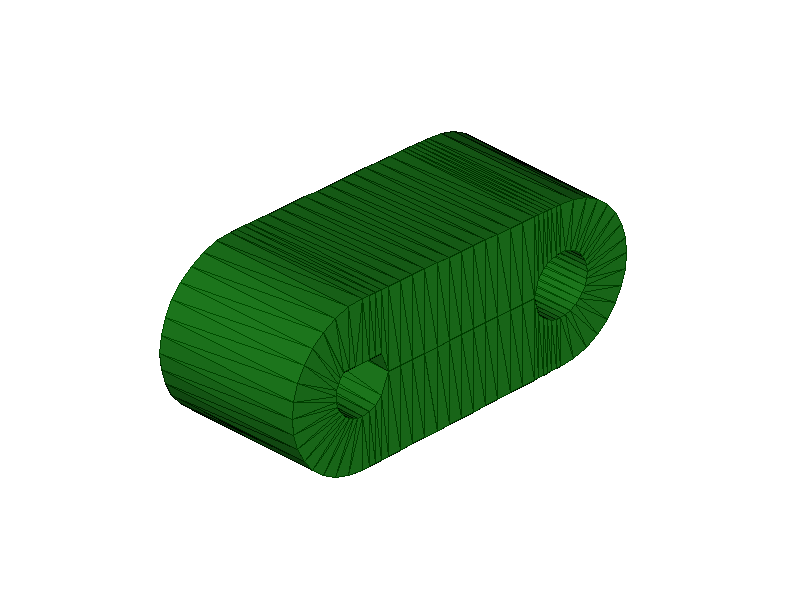
\includegraphics[width=0.70\textwidth]{figures/fig_rotor_arm_fab01.png}
\caption{Monolithic 3D-printed eccentric rotor cam arm (FAB-01) with calibrated D-shaft hub}
\label{fig:rotor_arm}
\end{figure}

The FAB-01 design incorporates the following precision mechanical features:
\begin{itemize}
    \item \textbf{Shrinkage-Compensated D-Shaft Bore:} FDM 3D printing in Polylactic Acid (PLA) exhibits approximately 1.5\% thermal radial shrinkage upon cooling. To guarantee a snug, zero-backlash press-fit over the nominal 3.00\,mm motor shaft without requiring manual reaming, the CAD bore is modeled with a 3.15\,mm circular diameter and a 2.65\,mm flat-to-back chord depth.
    \item \textbf{Eccentric Moment Arm:} Features a precision 12.0\,mm center-to-center radial pitch between the motor shaft center and the mass counter-recess hole.
    \item \textbf{Calibrated Unbalance Bolt Provision:} The outer extremity incorporates a 3.2\,mm through-hole with a counter-bored recess designed to receive an M3 steel unbalance bolt, dual steel washers, and a nylon locknut ($m_{\mathrm{unbalance}} \approx 1.85\,\text{g}$). When rotated at 600\,RPM (10\,Hz), this unbalance mass generates a repeatable rotating centrifugal unbalance force:
    \begin{equation}
    F = m \cdot r \cdot (2\pi f)^2 = (0.00185\,\text{kg}) \cdot (0.012\,\text{m}) \cdot (2\pi \cdot 10\,\text{rad/s})^2 = 0.0876\,\text{N}
    \end{equation}
    This dynamic force provides a perfectly controlled, repeatable mechanical anomaly for classifier evaluation.
\end{itemize}

\section{3D-Printed Rigid Sensor Mount (FAB-02) and Motor Shim (FAB-03)}
\subsection{High-Rigidity Sensor L-Bracket (FAB-02)}
Accelerometer mounting stiffness directly influences the usable measurement bandwidth. A flexible sensor bracket acts as a mechanical spring-mass filter, attenuating high-frequency vibrations and introducing spurious structural resonances.

Figure~\ref{fig:sensor_mount} illustrates the certified monolithic sensor mount (\textbf{FAB-02}).

\begin{figure}[H]
\centering
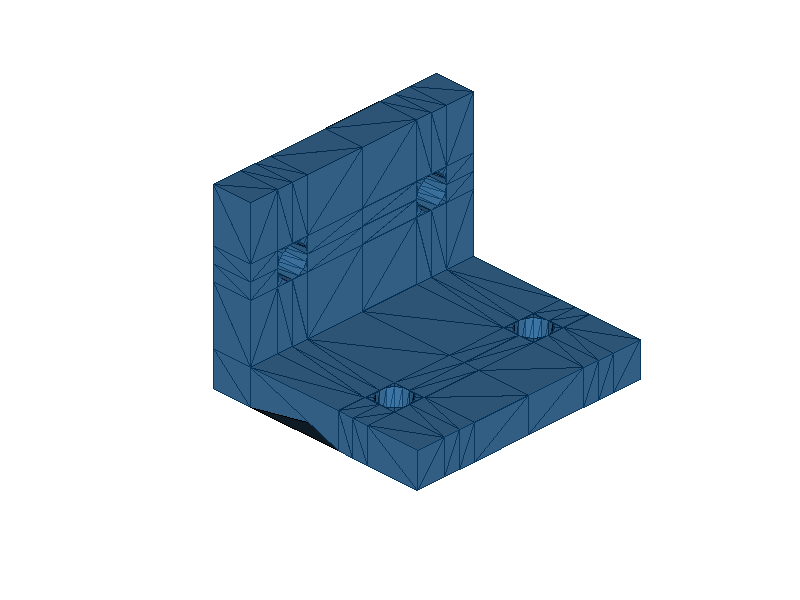
\includegraphics[width=0.70\textwidth]{figures/fig_sensor_mount_fab02.png}
\caption{Monolithic 3D-printed high-rigidity sensor mounting bracket (FAB-02)}
\label{fig:sensor_mount}
\end{figure}

FAB-02 is engineered with:
\begin{itemize}
    \item \textbf{Dual Triangular Stiffening Gussets:} Connect the 3.5\,mm thick vertical upright wall to the 4.0\,mm horizontal base flange, pushing structural bending resonance modes above 1,200\,Hz (far outside the 400\,Hz Nyquist measurement band).
    \item \textbf{Vertical Mounting Holes:} Spaced 15.0\,mm apart with 3.2\,mm clearance to rigidly clamp the Robocraze ADXL345 breakout PCB using M3 nylon hardware.
    \item \textbf{Base Flange Holes:} Spaced 15.0\,mm apart to anchor the bracket to the acrylic baseplate through-holes.
\end{itemize}

\subsection{Motor Bed Shim Pad (FAB-03)}
Due to the stamped metal construction of commercial N20 motor brackets, a slight 0.8\,mm gap exists between the cylindrical motor casing and the flat mounting surface. If tightened directly onto acrylic, the motor body cantilevers, creating an acoustic cavity that rattles at harmonics of gear mesh. To eliminate this noise, a custom 1.0\,mm thick PLA shim pad (\textbf{FAB-03}) was modeled and printed to support the motor belly, establishing a true co-planar, vibration-damped motor cradle.

\section{Fastener Sizing, Through-Bolting, and Isolation}
To prevent fastener loosening caused by continuous 10\,Hz cyclic vibration:
\begin{itemize}
    \item \textbf{Through-Bolted Clamping:} Rather than tapping threads directly into soft 10\,mm acrylic (which strips under cyclic shear), all 3.0\,mm holes pass through the full thickness of the baseplate. Fasteners are clamped on the bottom surface using M3 zinc-plated steel machine screws, wide flat washers, and nylon-insert locknuts (Nyloc).
    \item \textbf{Silicone Damping Feet:} Four 15\,mm diameter hemispherical silicone rubber damping pads are bolted to the corner datum holes. These pads isolate the testbed from the laboratory workbench, preventing external table vibrations from contaminating experimental data.
\end{itemize}

\section{Complete Bill of Materials (BOM) and Budget Realization}
Table~\ref{tab:bom} summarizes the finalized Bill of Materials, procurement channels, and financial ledger for the VibeGuard hardware realization.

\begin{table}[H]
\centering
\small
\begin{tabular}{|l|l|l|c|r|}
\hline
\textbf{Item Description} & \textbf{Component / SKU} & \textbf{Source / Channel} & \textbf{Qty} & \textbf{Cost (\rupee)} \\
\hline
Microcontroller Board & 7Semi ESP32-DEVKIT-E & Robocraze (Order 3) & 1 & 705.00 \\
Triaxial Accelerometer & ADXL345 MEMS Breakout & Robocraze (Order 1 \#TJFKQXJUQ) & 1 & 189.00 \\
Drive Motor & 12V N20 Gear Motor (600 RPM) & Robocraze (Order 1 \#TJFKQXJUQ) & 1 & 249.00 \\
Power Supply & 12V 2A DC SMPS Adapter & Robocraze (Order 1 \#TJFKQXJUQ) & 1 & 249.00 \\
Safety Disconnect & KCD1 SPST Rocker Switch & Robu.in (Order 2) & 1 & 25.00 \\
Overcurrent Protection & 1A 250V Fuses + Inline Holder & Robu.in (Order 2) & 2 & 65.00 \\
Inductive Clamping & 1N4007 Diodes (Pack) & College Lab Requisition & 2 & 0.00 \\
Decoupling Network & 100\,$\mu$F 25V + 100\,nF Ceramic & College Lab Requisition & 2 & 0.00 \\
Visual Indicator & Common-Cathode RGB LEDs & Robocraze (Order 1 \#TJFKQXJUQ) & 5 & 45.00 \\
Current Limiting & 330\,$\Omega$ 1/4W Metal Film Resistors & Robu.in (Order 2) & 10 & 20.00 \\
Baseplate Substrate & 10mm Laminated Acrylic Sheet & Mech Workshop Requisition & 1 & 0.00 \\
3D Printed Rotor (FAB-01) & PLA Monolithic Rotor Arm & Campus FabLab Requisition & 1 & 0.00 \\
3D Printed Mount (FAB-02) & PLA Rigid Sensor L-Bracket & Campus FabLab Requisition & 1 & 0.00 \\
Hardware Fasteners & M3 Screws, Nuts, Washers & Mech Workshop Requisition & 16 & 0.00 \\
Shipping & Bluedart Air / Courier Charges & Multi-vendor Shipping & -- & 374.00 \\
\hline
\multicolumn{4}{|l|}{\textbf{Total Project Expenditure}} & \textbf{\rupee 2,124.00} \\
\multicolumn{4}{|l|}{\textbf{Institutional Budget Ceiling}} & \textbf{\rupee 3,000.00} \\
\multicolumn{4}{|l|}{\textbf{Remaining Financial Reserve}} & \textbf{\rupee 876.00} \\
\hline
\end{tabular}
\caption{VibeGuard finalized multi-channel Bill of Materials (BOM) and financial ledger}
\label{tab:bom}
\end{table}

\section{Summary}
This chapter detailed the physical and mechanical implementation of VibeGuard. The 7Semi ESP32-DEVKIT-E provides dual-core processing power and breadboard clearance. The ADXL345 was configured in Full-Resolution $\pm 4g$ mode with a constant $3.9\,\text{mg/LSB}$ scale factor and 32-level FIFO buffering. The mechanical testbed was constructed on a 10\,mm laminated acrylic plate with precision dual-datum drilling coordinates. Monolithic 3D-printed parts (FAB-01, FAB-02, and FAB-03) resolved earlier structural separation failures, eliminated motor bracket rattle, and provided calibrated mechanical unbalance forces. Finally, the project financial ledger confirmed total hardware expenditure of \rupee 2,124.00, well within the \rupee 3,000 budget ceiling.
